\documentclass[a4paper]{scrartcl}
\usepackage[english]{babel}
\usepackage[top=2cm,bottom=3cm,left=2.5cm,right=2.5cm]{geometry}
\usepackage[colorlinks=true, allcolors=black]{hyperref}
\usepackage{wrapfig} %문단 내 이미지 삽입
\usepackage{graphicx} %색상
\usepackage{overpic}
\usepackage[normalem]{ulem}%취소선
\usepackage{array} %표
\usepackage{mdframed, tcolorbox} %글상자
\usepackage[yyyymmdd]{datetime}
	\renewcommand{\dateseparator}{--}
\usepackage{amsmath, amsfonts, amssymb, bm} %수식
	\DeclareMathOperator{\arccsc}{arccsc}
	\DeclareMathOperator{\arcsec}{arcsec}
	\DeclareMathOperator{\arccot}{arccot}
	\DeclareMathOperator{\csch}{csch}
	\DeclareMathOperator{\sech}{sech}
	\DeclareMathOperator{\arcsinh}{arcsinh}
	\DeclareMathOperator{\arccosh}{arccosh}
	\DeclareMathOperator{\arctanh}{arctanh}
	\DeclareMathOperator{\arccsch}{arccsch}
	\DeclareMathOperator{\arcsech}{arcsech}
	\DeclareMathOperator{\arccoth}{arccoth}
	
	\DeclareMathOperator{\meter}{m}
	\DeclareMathOperator{\cm}{cm}
	\DeclareMathOperator{\mm}{mm}
	\DeclareMathOperator{\mum}{\mu m}
	\DeclareMathOperator{\newton}{N}
	\DeclareMathOperator{\kn}{kN}
	\DeclareMathOperator{\kgf}{kgf}
	\DeclareMathOperator{\pa}{Pa}
	\DeclareMathOperator{\kpa}{kPa}
	\DeclareMathOperator{\mpa}{MPa}
	\DeclareMathOperator{\gpa}{GPa}
	\DeclareMathOperator{\npm}{N/m}
	\DeclareMathOperator{\knpm}{kN/m}
	\DeclareMathOperator{\kph}{km/h}
	\DeclareMathOperator{\mps}{m/s}
	\DeclareMathOperator{\tkph}{kph}
	\DeclareMathOperator{\tmps}{mps}
	\DeclareMathOperator{\mpss}{m/s^2}
	\DeclareMathOperator{\dgr}{\!^\circ}
	\DeclareMathOperator{\cel}{\!^\circ C}
	\DeclareMathOperator{\kg}{kg}
	\DeclareMathOperator{\kgpcm}{kg/m^3}
	\DeclareMathOperator{\nm}{N\cdot m}
	\DeclareMathOperator{\knm}{kN\cdot m}
	\DeclareMathOperator{\kw}{kW}
	\DeclareMathOperator{\kwh}{kWh}
	\DeclareMathOperator{\mmhg}{mmHg}
	\DeclareMathOperator{\snd}{s}
	
	\DeclareMathOperator{\joule}{J}
	\DeclareMathOperator{\jpcm}{J/m^3}
	\DeclareMathOperator{\mjpcm}{MJ/m^3}
\usepackage{polynom} %나눗셈 필산
\usepackage{cancel} %수식 약분선
\usepackage{titlesec} %섹션 이름 변경
	\titlespacing*{\section}{3mm}{0mm}{1mm}
	\titleformat{\section}{\bfseries\large}{}{0ex}{}
\usepackage{kotex} %한글

\newcommand{\prob}[2]{\section{#1}\begin{mdframed}#2\end{mdframed}}

\newlength{\picwidth}
\newcommand{\probpic}[4]{
	\setlength{\picwidth}{145mm}\addtolength{\picwidth}{-#3}\section{#1}\begin{mdframed}\begin{tabular}{m{#3}m{\picwidth}}
	\includegraphics[width = #3]{#2} & #4\end{tabular}\end{mdframed}
	}
	
\newcommand{\asw}[2]{
	\begin{flushright}
		#1\quad$\blacktriangleleft$\quad#2
	\end{flushright}
}

\newcommand{\aswtag}[1]{
	\quad\blacktriangleleft\quad#1
}

\title{\vspace{100pt}\Huge{HW6}}
\author{
	2025-2 구조역학(박성훈 교수님)\\[10pt]
	Problem 11.7, 11.15, 11.30, 11.34, 11.42, 11.45, 11.50, 11.59\\[100pt]
	오류 제보\quad eusnoohong03@soongsil.ac.kr\\
	}
\date{\today}

\begin{document}
	
\renewcommand*{\titlepagestyle}{empty}
\maketitle

\vspace{60pt}

\begin{center}
	\includegraphics[width=0.45\textwidth]{SSU symbol KR-EN.jpg}
\end{center}

\newpage\setcounter{page}{1}

\setlength{\parindent}{0pt}

\probpic{Problem 11.7}{img/P07.png}{85mm}{The load-deformation diagram shown has been drawn from data obtained during a tensile test of a specimen of an aluminum alloy. Knowing that the cross-sectional area of the specimen was $600\mm^2$ and that the deformation was measured using a 400-mm gage length. determine by approximate means ($a$) the modulus of resilience of the alloy, ($b$) the modulus of toughness of the alloу.}

\begin{align*}
	&\sigma_Y = \frac{P_Y}{A} = \frac{300\times10^3}{600\times10^{-6}}\pa = 500\mpa\\
	&\varepsilon_Y = \frac{\delta_Y}{L} = \frac{2.8}{400} = 0.007\\
	&(\text{modulus of resilience}) = \frac{1}{2}\sigma_Y\varepsilon_Y = \frac{1}{2}(500\times10^6)(0.007)\jpcm = 1.750\mjpcm\aswtag{(a)}\\
	&\varepsilon_R = \frac{\delta_R}{L} = \frac{50}{400} = 0.125\\
	&P_\text{avg} \approx 350\kn\quad\Rightarrow\quad \sigma_\text{avg} \approx \frac{350\times10^3}{600\times10^{-6}}\pa = 583.333\mpa\\
	&(\text{modulus of resilience}) = \sigma_\text{avg}\varepsilon_R \approx (583.333\times10^6)(0.125)\jpcm = 72.9\mjpcm\aswtag{(b)}
\end{align*}

\newpage

\probpic{Problem 11.15}{img/P15.png}{65mm}{Rod $ABC$ is made of a steel for which the yield strength is $\sigma_Y = 450\mpa$ and the modulus of elasticity is $E = 200\gpa$. Knowing that a strain energy of $11.2\joule$ must be acquired by the rod as the axial load $P$ is applied, determine the factor of safety of the rod with respect to permanent deformation when $a = 0.5\meter$.}

\begin{align*}
	&A_{AB} = \pi(0.009)^2\meter^2 = 2.54469\times10^{-4}\meter^2,\quad A_{BC} = \pi(0.006)^2\meter = 1.130973\times10^{-4}\meter^2\\
	&P_Y = \sigma_YA_{BC} = (450\times10^6)(1.130973\times10^{-4}) = 50.8938\kn\\
	&U_Y = \frac{P_Y^2L_{AB}}{2EA_{AB}} + \frac{P_Y^2L_{BC}}{2EA_{BC}} = \frac{P_Y^2}{2E}\left(\frac{L_{AB}}{A_{AB}} + \frac{L_{BC}}{A_{BC}}\right)\\
	&\phantom{U_Y} = \frac{50893.8^2}{2(200\times10^9)}\left(\frac{0.8}{2.54469\times10^{-4}} + \frac{0.5}{1.130973\times10^{-4}}\right)\joule = 48.9853\joule\\
	&(F.S.) = \frac{U_Y}{U} = \frac{48.9853\joule}{11.2\joule} = 4.37\aswtag{}
\end{align*}

\vspace{20pt}

\probpic{Problem 11.30}{img/P30.png}{60mm}{Using $E = 200\gpa$, determine the strain energy due to bending for the steel beam and loading shown. (Neglect the effect of shearing stresses.)}
\includegraphics{img/fig001.png}
\begin{align*}
	&I = 178\times10^{6}\mm^4 = 178\times10^{-6}\meter^4\\
	&\int^L_0 M^2dx = A_{m^2} = \frac{1}{3}(46656)(4.8)\kn^2\cdot\meter^3 = 74649.6\kn^2\cdot\meter^3\\
	&U = \int^L_0 \frac{M^2}{2EI}dx = \frac{A_{m^2}}{2EI} = \frac{74649.6\times10^6}{2(200\times10^9)(178\times10^{-6})}\joule = 1048\joule\aswtag{}
\end{align*}

\newpage

\probpic{Problem 11.34}{img/P34.png}{85mm}{Two solid shafts are connected by the gears shown. Using $G = 77\gpa$, determine the strain energy of each shaft when a 2.7-kN-m. torque $T$ is applied at $D$. (Ignore the strain energy due to bending of the shafts.)}
\begin{align*}
	&T_{AB} = \frac{200\mm}{125\mm}(2.7\knm) = 4.32\knm,\quad T_{CD} = 2.7\knm\\
	&J_{AB} = \frac{\pi}{2}(0.025)^4\meter^4 = 9.65499\times10^{-7}\meter^4\\
	&J_{CD} = \frac{\pi}{2}(0.025)^4\meter^4 = 6.13592\times10^{-7}\meter^4\\
	&U = \frac{T_{AB}^2L_{AB}}{2GJ_{AB}} + \frac{T_{CD}^2L_{CD}}{2GJ_{CD}} = 120.6\joule\aswtag{}
\end{align*}

\vspace{20pt}

\probpic{Problem 11.42}{img/P42.png}{70mm}{A 5-kg collar $D$ moves along the uniform rod $AB$ and has a speed $V = 6\mps$ when it strikes a small plate attached to end $A$ of the rod. Using $E = 200\gpa$ and knowing that the allowable stress in the rod is $250\mpa$, determine the smallest diameter that can be used for the rod.}
\begin{align*}
	&U = \frac{1}{2}mv_0^2 = \frac{1}{2}(5)(6^2)\joule = 90\joule\\
	&P_\text{all} = \sigma_\text{all} A,\quad A = \frac{\pi}{4}d^2\\
	&U \leq U_\text{all} = \frac{P_\text{all}^2L}{2EA} = \frac{\sigma_\text{all}^2AL}{2E} = \frac{\pi\sigma_\text{all}^2d^2L}{8E}\\
	&d \geq \sqrt{\frac{8UE}{\pi\sigma_\text{all}^2L}} = \sqrt{\frac{8(90)(200\times10^9)}{\pi(250\times10^6)^2(1.2)}}\meter = 24.7\mm\aswtag{}
\end{align*}

\newpage

\probpic{Problem 11.45}{img/P45.png}{55mm}{Сollar $D$ is released from rest in the position shown and is stopped by a small plate attached at end $C$ of the vertical rod $ABC$. Determine the mass of the collar for which the maximum normal stress in portion $BC$ is $125\mpa$.}
\begin{align*}
	&A_{AB} = \pi(0.006)^2\meter^2 = 1.130973\times10^{-4}\meter^2\\
	&A_{BC} = \pi(0.0045)^2\meter^2 = 6.36173\times10^{-5}\meter^2\\
	&P_m = \sigma_mA_{BC} = 7952.16\newton\quad(\because A_\text{min} = A_{BC})\\
	&U_m = \frac{1}{2}P_m\delta_m = \frac{P_m^2L_{AB}}{2E_bA_{AB}} + \frac{P_m^2L_{BC}}{2E_aA_{BC}}\quad\Rightarrow\quad \delta_m = P_m\left(\frac{L_{AB}}{E_bA_{AB}} + \frac{L_{BC}}{E_aA_{BC}}\right) = \frac{1}{140}\meter\\
	&U \leq U_m\quad\Rightarrow\quad mg(h+\delta_m) \leq \frac{1}{2}P_m\delta_m \quad\Rightarrow\quad m \leq \frac{P_m\delta_m}{2g(h+\delta_m)} = 4.77\kg\aswtag{}
\end{align*}

\newpage

\probpic{Problem 11.50}{img/P50.png}{80mm}{An aluminum tube having the cross section shown is struck squarely in its midsection by a 6-kg block moving horizontally with a speed of $2\mps$. Using $E = 70\gpa$, determine ($a$) the equivalent static load, ($b$) the maximum stress in the beam, ($c$) the maximum deflection at the midpoint $C$ of the beam.}
$$U = \frac{1}{2}mv_0^2 = \frac{1}{2}(6)(2^2)\joule = 12\joule$$
\includegraphics{img/fig002.png}
\begin{align*}
	&L = 1.8\meter,\quad M_C = \frac{P}{2}\cdot\frac{L}{2} = \frac{PL}{4}\\
	&\int^L_0 M^2dx = A_{m^2} = \frac{1}{3}\left(\frac{P^2L^2}{16}\right)L = \frac{P^2L^3}{48}\\
	&I = \frac{1}{12}\left\{(0.08)(0.1)^3 - (0.06)(0.08)^3\right\}\meter^4 = 4.10667\times10^{-6}\meter^4\\
	&U = \int^L_0 \frac{M^2}{2EI}dx = \frac{A_{m^2}}{2EI} = \frac{P^2L^3}{96EI}\quad\Rightarrow\quad P = \sqrt{\frac{96UEI}{L^3}} = 7535.49\newton = 7.54\kn\aswtag{(a)}\\
	&\sigma_m = \frac{|M|_mc}{I} = \frac{PLc}{4I} = 41.3\mpa\aswtag{(b)}\\
	&U = \frac{1}{2}Py_C\quad\Rightarrow\quad y_C = \frac{2U}{P} = 3.18\mm\aswtag{(c)}
\end{align*}

\newpage

\probpic{Problem 11.59}{img/P59.png}{55mm}{Using the method of work and energy, determine the deflection at point $D$ caused by the load $\mathbf{P}$.}
\begin{align*}
	&+\circlearrowleft\sum M|_A = Pa - R_BL = 0,\quad R_B = \frac{Pa}{L}\\
	&+\uparrow\sum F_y = -P - R_B + R_A = 0,\quad R_A = P\left(1+\frac{a}{L}\right)
\end{align*}
\includegraphics{img/fig003.png}
\begin{align*}
	&\int^L_0 M^2dx = A_{m^2} = \frac{1}{3}P^2a^2(a+L)\\
	&U = \int^L_0\frac{M^2}{2EI}dx = \frac{A_{m^2}}{2EI} = \frac{P^2a^2(a+L)}{6EI} = \frac{1}{2}P|y_D|\quad\Rightarrow\quad y_D = -\frac{Pa^2(a+L)}{3EI}\aswtag{}
\end{align*}

\end{document}